\subsection{Beslutningsproblemer og stand-in sprog}
\subsection{P, NP, NPC}
\subsection{Reduktioner}
\subsection{3SAT $\le$ HAMILTONIAN PATH}
\textbf{Theorem 9.7:} HAMILTONIAN PATH is NP-Complete\\\\
We prove this by reducing from 3SAT, which we know is NP-complete.\\\\
We construct a graph G such that G has a Hamiltonian path if and only if the input 3sat formula has a satisfying assignment.\\\\
For each variable we add a choice gadget and join them. For each clause we add a triangle where each edge corresponds to a literal in the clause. For each edge in the triangle, we add a consistency gadget from the edge, to the edge in the corresponding choice gadget. All nodes in all triangles belong to a clique together with the edge following the last choice gadget, and some other node which is the only one adjacent to the last edge in our path (see figure 6.)\\\\
The important thing is that all triangle have at least one edge visited (or actually the 4 nodes on the edges) by the time we get to the clique member after the last choice gadget. If this is not the case then we cannot visit all nodes in a triangle without visiting one of the clique members twice. Recall that edges in the triangles represent literals in the clause - the edges we visit via the choice gadgets are the one for which the corresponding literal make the clause true, and so if no edge is visited, then the clause is false. This is consistent with the fact that we cannot make a hamiltonian cycle. \\\\
Figure 5 show exactly what happens with the consistency gadget. Our path goes through nodes 1,2,3,4... and leaves at 12. It is clear that none of the black nodes are visited. \\\\
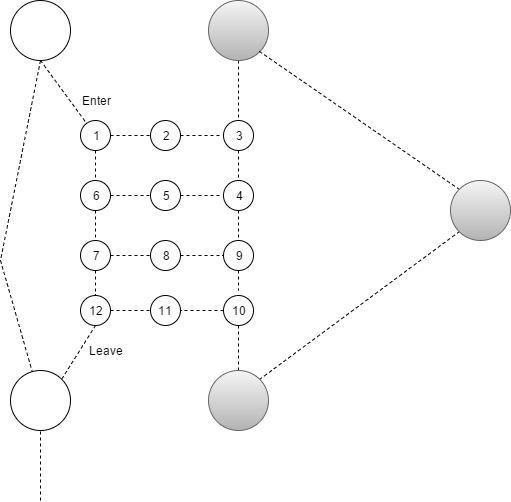
\includegraphics[scale=0.5]{HAMConsistency}\\
\textbf{Figure 5:} Zooming in on the consistency gadget between the choice gadget and the triangle.\\\\
\textbf{Example:}\\
Given a 3SAT formula  $f = (x_1 \lor x_2 \lor x_3) \land (\lnot x_1 \lor \lnot x_2 \lor x_3) \land (\lnot x_1 \lor \lnot x_2 \lor x_3)$\\
We can construct a graph similar to the one in figure 6. For the satisfying assignment $x_1 = 1, x_2 = 0, x_3 = 0$, we can obtain a hamiltonian path by starting at 1, and follwing the pink line to 2.
\begin{center}
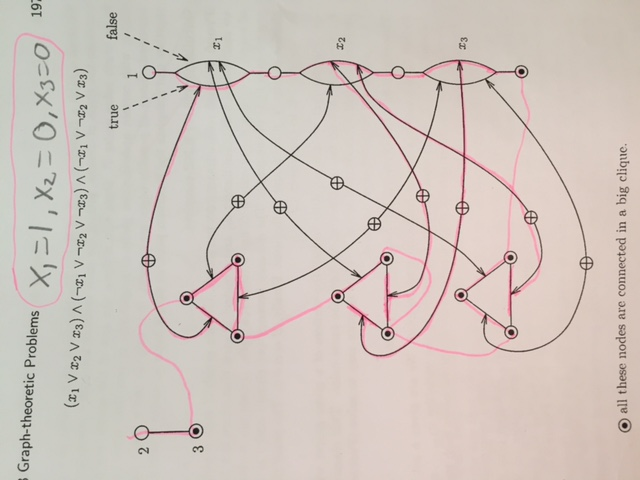
\includegraphics[scale=0.5, angle =-90]{3SATtoHAM}\\
\textbf{Figure 6:} Graph r(f) corresponding to the formula f
\end{center}
\textbf{Polynomial time reduction:}\\
For each variable we make one choice gadget, and for each clause we make one triangle and 3 consistency gadgets.\\\\
$\implies$: \\
Given a satisfying assignment to the input formula f we can show that r(f) has a hamiltonian path: Simply follow the path though the choice gadgets which corresponds to the truth value of the variables. When reaching the clique node after the last choice gadget, we just jump around in the clique and travers the missing edges in each triangle and finally jump to node 3 and then finally 2. 
$\impliedby$: \\
Given that the graph has a hamiltonian path, we show that the input formula is satisfiable: Since there is only two nodes with degree one we can assume the path starts at node 1. Since we know the structure of the graph and the the given hamiltonian path, a truth assignment T is defined by the way the path traverse the choice gadgets and the consistency gadgets along the way. T satisfies the input formula.
\newpage
\subsection{HAMILTONIAN PATH $\le$ TSP}
//TODO

\subsection{3SAT $\le$ INDEPENDENT SET}
\textbf{Theorem 9.4:} INDEPENDENT SET is NP-Complete\\\\
We prove this by reducing from 3SAT, which we know is NP-Complete.\\\\
For this reduction we need a gadget, the triangle. The logic behind this is that, if a graph contains a triangle, then at most one of the nodes can be in the independent set. We restrict the class of graphs we consider, to graphs whose nodes can be partitioned in m disjoint triangles. This ensures that an independent set can contain at most m nodes. \\

For each of the m clauses in our input CNF formula, we create a triangle where the nodes are labeled with the literals of the clause. Next, we add an edge between two nodes in different triangles if and only if the nodes correspond to opposite literals. Adding these edges between opposite literals, ensures that we cannot pick both (as it would not be an independent set). The reduction is completed by setting the independent set goal K = m. \\\\\\
\textbf{Example:}\\
Given a 3CNF formula:  $f =  (x_1 \lor x_2 \lor x_3) \land (\lnot x_1 \lor \lnot x_2 \lor \lnot x_3) \land (\lnot x_1 \lor x_2 \lor x_3)$\\
We construct the graph shown in figure 1. \\\\
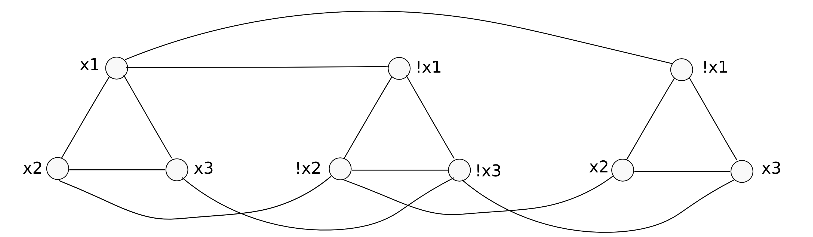
\includegraphics[scale=0.5]{independentset}
\textbf{Figure 1:} Graph r(f) corresponding to the formula f\\\\\\
\textbf{Analysis}\\
For each clause, we just create a triangle. Then we scan every pair of edges and add an edge if the labels are opposite - so the reduction is clearly polynomial.
\\\\
$\implies$ :\\ Given a satisfying assignment for the CNF formula f from above, we must show that the graph, r(f), has an indenpendent set of size K=m. The assignment: $x_1 = 0, x_2 = 1, x_3 = 0$ satisfies the formula, and for our independent set of size K, we pick a node in each triangle which make the corresponding clause true. For the truth assignment we chose above, this means $x_2$ from triangle 1, $\lnot x_1$ in triangle 2, $\lnot x_1$ in triangle 3. (Note that this is not the only valid set since some clauses are satisfied by more than one literals).
\\\\
$\impliedby$ :\\ Given an independent set of size K of r(f), we need to show that there is a satisfying assignment for f. Since it is of size K, it must have one vertex from each triangle, and it cannot contain a variable and its negation. Now, for each vertex in the independent set, we look at the label and assign a truth value to the corresponding variable, so the literal of the label become true. If a variable is not restricted to a truth value by any vertex label, we just assign it some value, since all clauses are already satisfied by the assignments to the other variables.\\\\\\
\textit{Read more in papadimitriou page 188-190.}
\newpage
\subsection{INDEPENDENT SET $\le$ CLIQUE}
The independent set problem asks for a maximum set of vertices of size K. So does the CLIQUE problem. While the independent set problem asks for a set S of vertices where there is no edge between any pair $u,v \in S$, the clique problem ask for the "opposite": a set S where any pair $u,v \in S$ DOES have an edge between them. So the reduction is trivial - we obtain a clique of size K when taking the complementary graph of an independent set of size K.\\\\
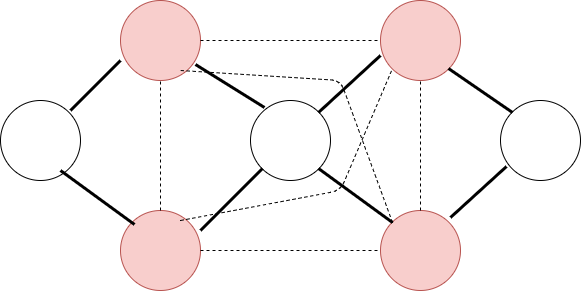
\includegraphics[scale=0.5]{IStoCLIQ}\\
\textbf{Figure 2:} The red nodes are the maximum independent set I - the dotted lines completes the complementary graph of I. A clique of same size.
\\\\\\
\textit{Read more in papadimitriou page 190.}
\newpage
\subsection{INDEPENDENT SET $\le$ VERTEX COVER}
While independent set is a maximization problem, vertex cover is a minimization problem. For a graph G = (V,E) and a max independent set $I \subseteq V$, the minimum vertex cover set is just $V-I$.\\\\
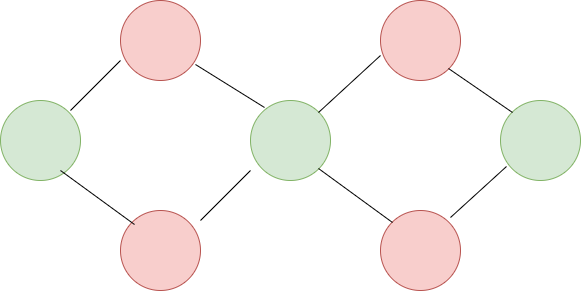
\includegraphics[scale=0.5]{IStoCOVER}\\
\textbf{Figure 3:} The red node forms the maximum independent set. The green form the minimal vertex cover.
\\\\\\
\textit{Read more in papadimitriou page 190.}
\newpage
